\section{Permission Regions}

\begin{figure}[t]
  \centering
  \scalebox{0.4}{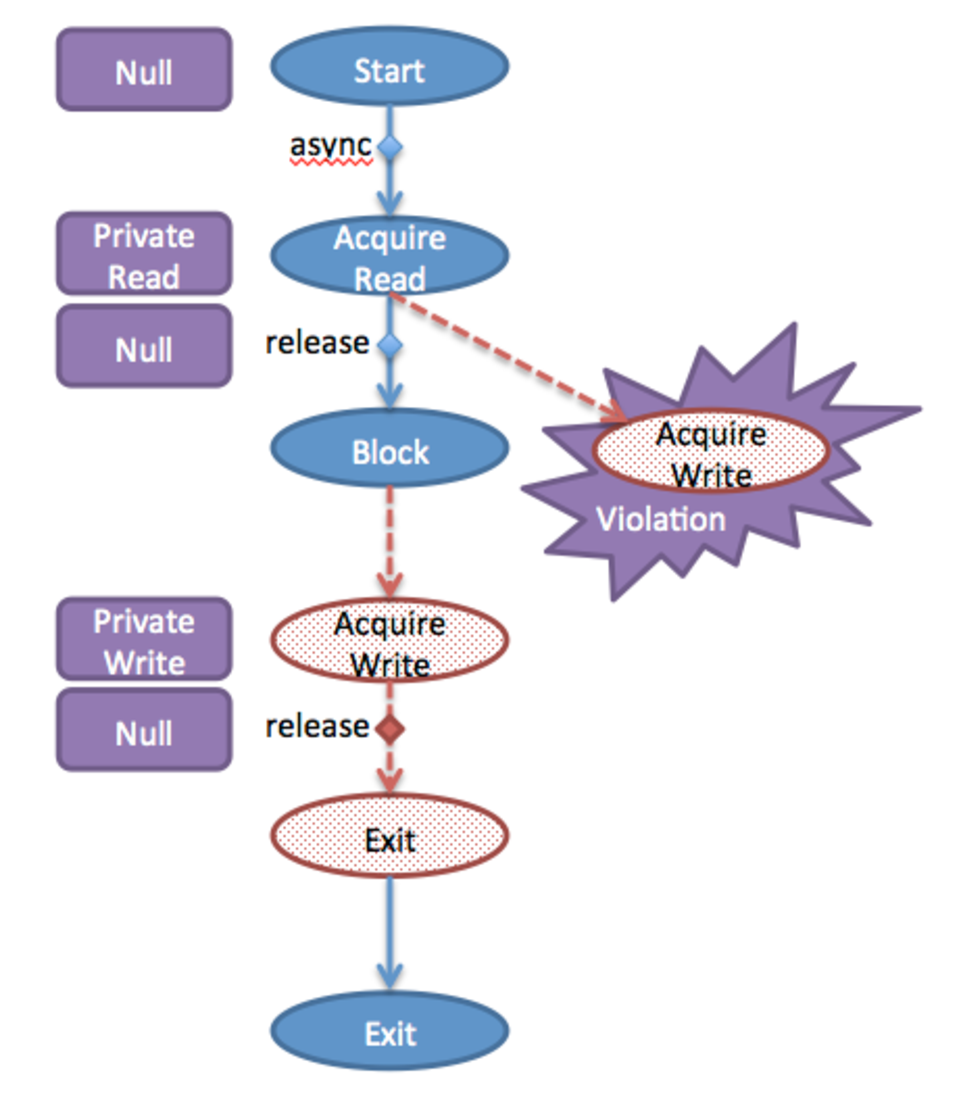
\includegraphics{../figs/stack-violation}}
  \caption{Different schedules for a permission region annotated
    version of the program in \figref{fig:hj-async-finish} with the
    schedule in the right branch reporting a permission violation.}
  \label{fig:permission-violation-state}
\end{figure}

Permission regions are programmer added annotations on shared objects
\cite{Westbrook:2011:PRR:2341616.2341627,Westbrook:2012:PPR:2367163.2367201}. The regions are indicated
as accessing shared objects in read or write mode. When the program
executes with run-time checking of permission regions enabled, a state machine is associated with each shared object to track
permissions on that object as indicated by the program annotations. If
accesses from distinct tasks on the same object conflict (i.e., a read
with a write or a write with a write), then a permission violation, indicative of a data race, is detected. An absence of violations implies an absence of any data races. 

To annotate the program in \figref{fig:hj-async-finish} with
permission regions, \lineref{line:push} and \lineref{line:peek} are
wrapped in separate regions, writing and reading, respectively, as follows:
\begin{lstlisting}
acquireW(stk);
stk.push(5);
releaseW(stk);
\end{lstlisting}
\begin{lstlisting}
acquireR(stk);
stk.peek();
releaseR(stk);
\end{lstlisting}
%Permission regions are transitive and span all the code in the
%\texttt{stk.push} and \texttt{stk.peek} methods.

The state machine associated with each region to track accesses and
detect violations is not shown due to space limitations, but it is intuitively
understood from the two possible task schedules in
\figref{fig:permission-violation-state} for an annotated version of the
program in \figref{fig:hj-async-finish}. The solid filled ovals and
solid lines represent the parent task and the dotted filled ovals and
dashed lines represent the child task created by the
\texttt{async}-statement on \lineref{line:async}. The squares indicate the current state of
the state machine that is tracking accesses to the shared object
\texttt{stk}.

The left branch of the tree is the schedule where the parent task runs
until it is blocked to wait for the child task. The parent task acquires
and releases private read privileges on the region and then the newly
created task runs, acquiring and releasing private write
privileges. If this schedule is followed in the run-time, then the
permission violation in the program is undetected. The right branch is another
possible schedule in the run-time. Here the child task runs just after
the parent task acquires private read privileges on {\tt stk}. When the
child task tries to acquire write privileges on {\tt stk}, its
state machine detects the violation.

Permission regions are distinctly different from mutual exclusion primitives such as locks and the Habanero 
\texttt{isolated}-construct. The \texttt{isolated}-construct defines
an atomic region that runs mutually exclusive to any other
\texttt{isolated}-construct and can be used to express  non-determination that is
intended by the programmer.  As such, isolated atomic regions are
serialized with respect to one another. Permission regions do not
include any serialization or synchronization semantics by themselves; rather, they check if concurrent accesses obey the permission annotations.
